O painel web foi construído com FastAPI no servidor e HTML, CSS e JavaScript
sem bibliotecas externas no navegador, para funcionar sem acesso à internet.
Ele lê exclusivamente dados produzidos pela aplicação: o estado escrito pelo
modo \emph{live} a cada passo, o banco SQLite alimentado pela ingestão MQTT,
um traço gravado de simulação e o resumo dos experimentos. Há três visões:

\begin{itemize}
  \item \textbf{Operação ao vivo} (Figura~\ref{fig:painel}a): mapa da malha
  viária com os contêineres coloridos pela ocupação estimada, contêineres sem
  dado recente em contorno, dispositivos \emph{offline} marcados, depósito,
  veículos e rotas do dia desenhadas pelas ruas; indicadores de distância,
  coletas, transbordamento, dispositivos \emph{online} e mensagens
  (recebidas, duplicadas e rejeitadas); filtros por estado; histórico de
  telemetria de cada contêiner, consultado no SQLite; e lista de eventos
  MQTT. Um seletor alterna entre o estado estimado pela plataforma e o estado
  verdadeiro do simulador, o que permite observar a diferença entre o que o
  operador vê e o que de fato ocorre.
  \item \textbf{\emph{Replay} A $\times$ D} (Figura~\ref{fig:painel}b):
  reprodução sincronizada de duas execuções com a mesma semente, com controle
  de tempo e velocidade.
  \item \textbf{Resultados}: tabela do experimento E1 e fronteira do E2, lidas
  do resumo gerado pela análise.
\end{itemize}

\begin{figure}[ht]
  \centering
  \begin{subfigure}{\textwidth}\centering
    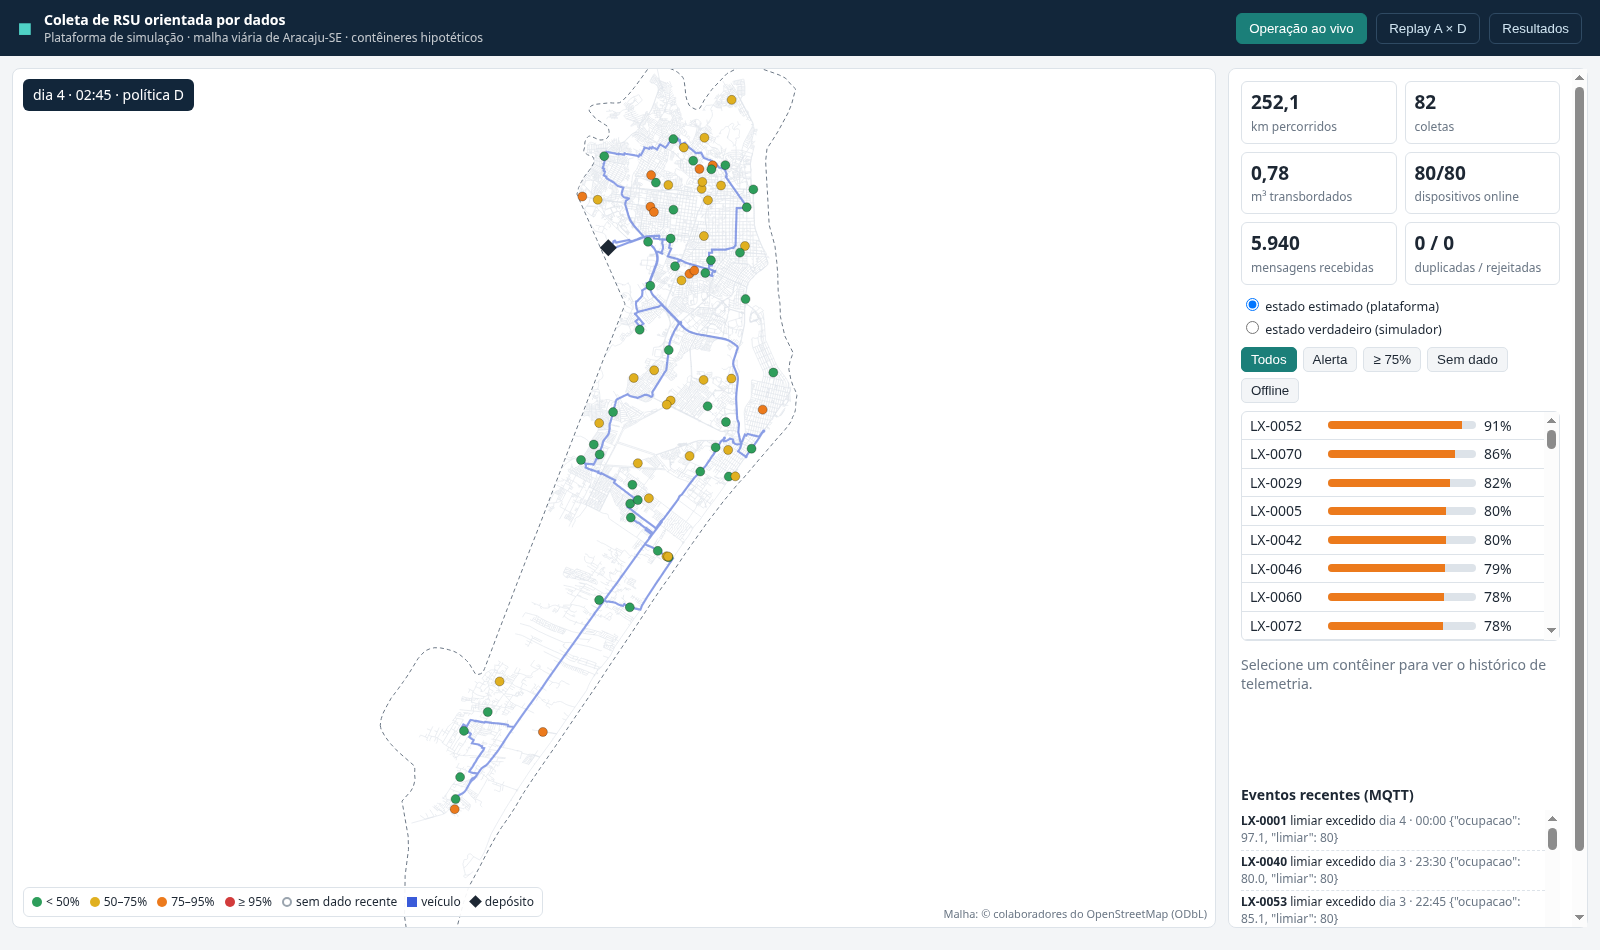
\includegraphics[width=0.93\textwidth]{figures/painel_ao_vivo.png}
    \caption{Operação ao vivo: telemetria recebida pelo broker, rotas do dia e histórico de um contêiner.}
  \end{subfigure}\\[4pt]
  \begin{subfigure}{\textwidth}\centering
    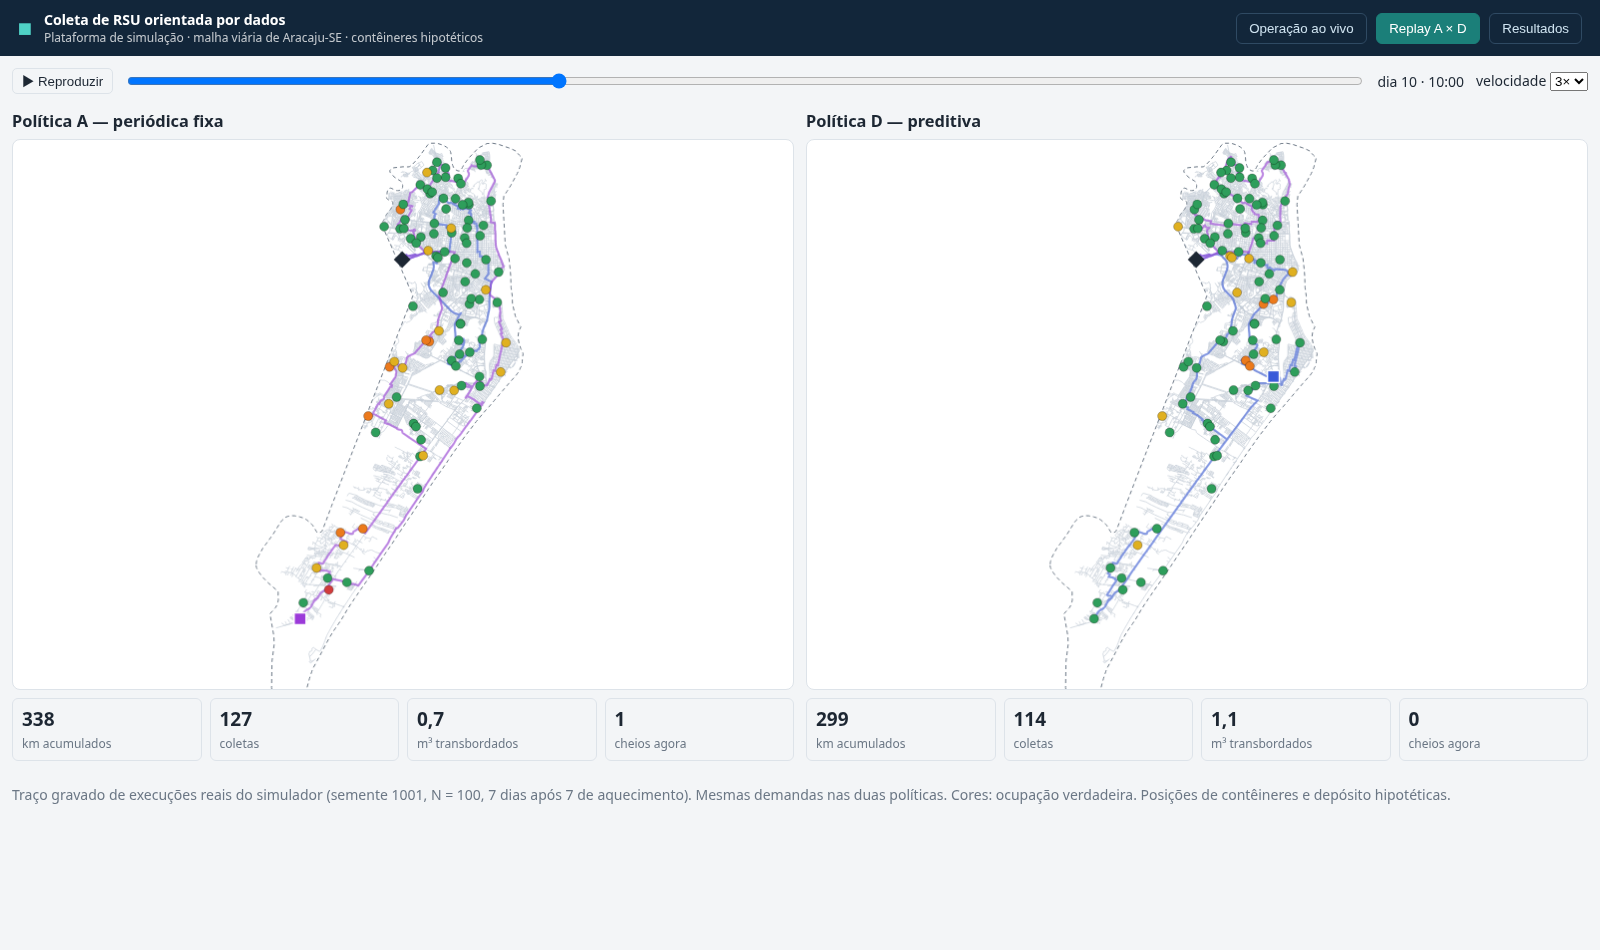
\includegraphics[width=0.93\textwidth]{figures/painel_replay.png}
    \caption{Replay sincronizado das políticas A e D (semente 1001, $N = 100$).}
  \end{subfigure}
  \caption{Capturas do painel operacional, obtidas com a aplicação em execução (navegador em modo \emph{headless}).}
  \label{fig:painel}
\end{figure}
